\begin{figure}[h] 
\centering 
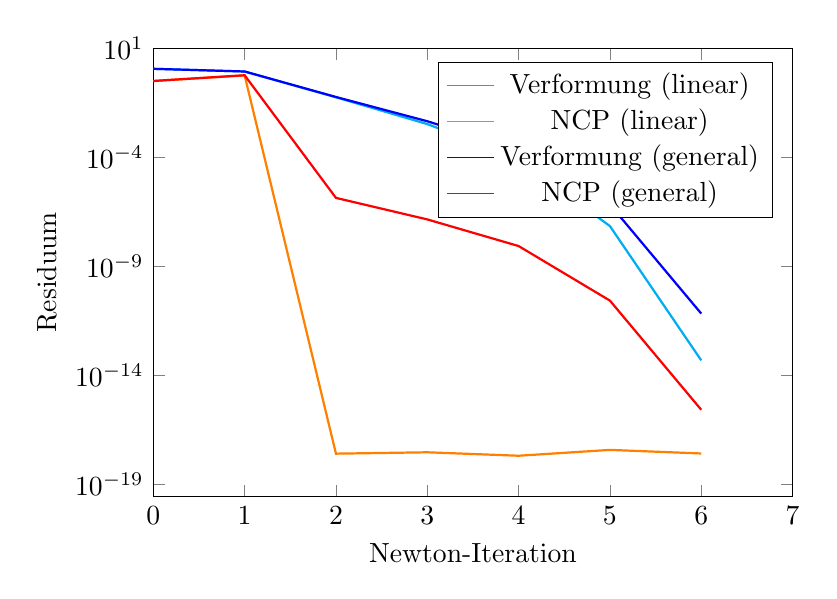
\begin{tikzpicture}[every plot/.append style={thick}] 
\begin{axis}[ 
label style={font=\normalsize}, 
xlabel={Newton-Iteration}, 
ylabel={Residuum}, 
xmin=0, xmax=7, 
ymode=log, 
ymin=0, ymax=10, 
width=0.8\textwidth, 
height=0.6\textwidth, 
legend pos=north east, 
legend style={cells={align=left}}, 
grid style=dashed, 
] 
\addplot[ 
color=cyan, 
] 
coordinates { 
(0, 1.13e+00)(1, 8.50e-01)(2, 5.57e-02)(3, 3.29e-03)(4, 8.36e-05)(5, 6.87e-08)(6, 4.74e-14)}; 
\addlegendentry{Verformung (linear)} 
\addplot[ 
color=orange, 
] 
coordinates { 
(0, 3.13e-01)(1, 5.62e-01)(2, 2.49e-18)(3, 2.88e-18)(4, 2.00e-18)(5, 3.71e-18)(6, 2.54e-18)}; 
\addlegendentry{NCP (linear)} 
\addplot[ 
color=blue, 
] 
coordinates { 
(0, 1.13e+00)(1, 8.50e-01)(2, 5.76e-02)(3, 4.44e-03)(4, 2.14e-04)(5, 6.72e-07)(6, 6.65e-12)}; 
\addlegendentry{Verformung (general)} 
\addplot[ 
color=red, 
] 
coordinates { 
(0, 3.12e-01)(1, 5.72e-01)(2, 1.35e-06)(3, 1.39e-07)(4, 8.35e-09)(5, 2.62e-11)(6, 2.57e-16)}; 
\addlegendentry{NCP (general)} 
\end{axis} 
\end{tikzpicture} 
\caption{Residuen des Stoffgesetzes 'St.Venant' mit Hinderniss 'Parabel' und 578 Freiheitsgraden für die Verschiebung.} 
\label{fiq:St.Venant_Parabel_level3} 
\end{figure} 
